\documentclass{standalone}
% translate with >> pdflatex -shell-escape <file>

% This file is an extract of the PGFPLOTS manual, copyright by Christian Feuersaenger.
% 
% Feel free to use it as long as you cite the pgfplots manual properly.
%
% See
%   http://pgfplots.sourceforge.net/pgfplots.pdf
% for the complete manual.
%
% Any required input files (for <plot table> or <plot file> or the table package) can be downloaded
% at
% http://www.ctan.org/tex-archive/graphics/pgf/contrib/pgfplots/doc/latex/
% and
% http://www.ctan.org/tex-archive/graphics/pgf/contrib/pgfplots/doc/latex/plotdata/

\usepackage{pgfplots}
\usepackage{pgfplotstable}
\pgfplotsset{compat=newest}

% The manual loads these libraries globally; the extracted standalone examples
% need them too. external/clickable/snakes are intentionally omitted.
\usetikzlibrary{
	arrows.meta,backgrounds,calc,decorations.footprints,decorations.markings,
	decorations.pathreplacing,fixedpointarithmetic,intersections,patterns,
	plotmarks,shapes.arrows,spy,through}
\usepgfplotslibrary{
	colorbrewer,colormaps,dateplot,fillbetween,groupplots,patchplots,polar,
	smithchart,statistics,ternary,units}

% Some colormap examples reuse this display style defined earlier in the manual.
\pgfplotsset{
	cycle from colormap manual style/.style={
		x=3cm,y=10pt,ytick=\empty,
		colorbar style={x=,y=,ytick=\empty},
		point meta min=0,point meta max=1,
		stack plots=y,
		y dir=reverse,colorbar style={y dir=reverse},
		every axis plot/.style={line width=2pt},
		legend entries={0,...,20},
		legend pos=outer north east,
	},
}

\pagestyle{empty}

\usepgfplotslibrary{ternary}

\begin{document}
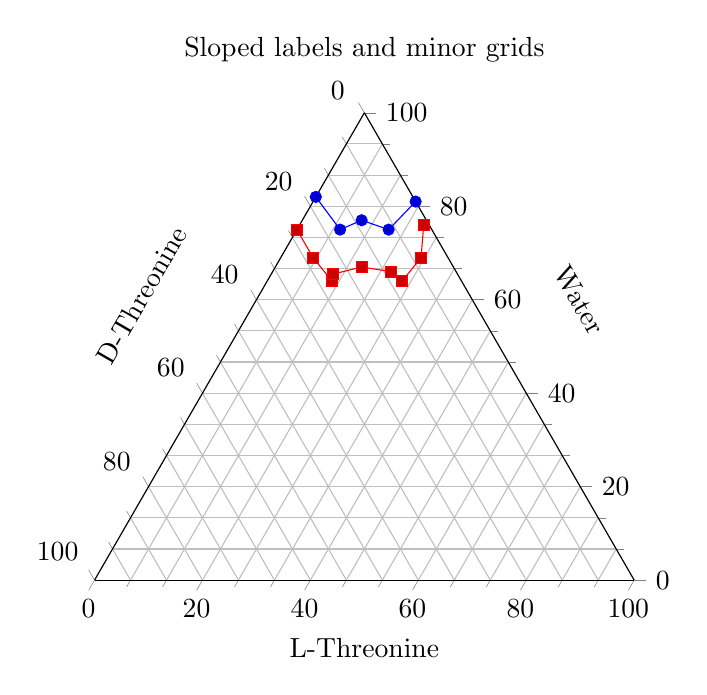
\begin{tikzpicture}
\begin{ternaryaxis}[
    title=Sloped labels and minor grids,
    xlabel=Water,
    ylabel=D-Threonine,
    zlabel=L-Threonine,
    label style={sloped},
    minor tick num=2,
    grid=both,
]
    \addplot3 coordinates {
        (0.82,  0.18,  0.00)
        (0.75,  0.17,  0.08)
        (0.77,  0.12,  0.11)
        (0.75,  0.08,  0.17)
        (0.81,  0.00,  0.19)
    };
    \addplot3 coordinates {
        (0.75,  0.25,  0.00)
        (0.69,  0.25,  0.06)
        (0.64,  0.24,  0.12)
        (0.655, 0.23,  0.115)
        (0.67,  0.17,  0.16)
        (0.66,  0.12,  0.22)
        (0.64,  0.11,  0.25)
        (0.69,  0.05,  0.26)
        (0.76,  0.01,  0.23)
    };
\end{ternaryaxis}
\end{tikzpicture}
\end{document}
